% !TeX root = ../thuthesis-example.tex

\chapter{基于特征关系图的循环神经网络算法}
\section{引言}
从第三章的实验可以知道,现有的异常检测算法能够在公开数据集取得较为不错的表现,但是在真实数据集——清华大学校园网流量数据上效果均无法达到要求。这是因为相比于人工构造的公开数据集,清华大学校园网数据具有规模大、应用类型种类繁多、异常流量占比多、难以学到基线等特点。现有的算法无论是传统机器学习的LR、NB、DT,还是拟合能力更强大的深度学习模型CNN、LSTM、GRU,都有精确率低、误报率高的问题。本章将先从特征分析着手,引入特征之间的关系矩阵,将其加入到神经网络的训练中,从而获得更好的检测效果。
\section{特征分析}
流量特征可以视为反映当前网络流量的一组观察值,从多个角度描述当前的流量场景。好的特征能够真实地反映出流本身的状态信息。例如对于一条单个TCP流,这条流可能是一个正常的端到端的链接,也可能是分布式拒绝服务攻击的一部分,在被攻击者的视角内,它的入流量的带宽急剧增加,且远大于出流量的带宽。图\ref{fig:特征关系}表示某一时刻下部分特征之间的关系,从中我们看出,发送方/接收方数据包长度大小与流的传输速率具有很强的关联性。

\begin{figure}
  \centering
  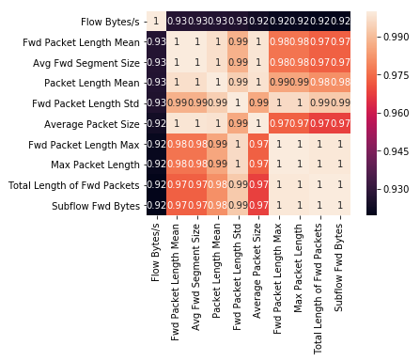
\includegraphics[scale=1]{特征关系.png}
  \caption{特征关系}
  \label{fig:特征关系}
\end{figure}

为了在神经网络中引入特征关系矩阵,本文利用皮尔逊相关系数来计算流量特征之间的关系。皮尔逊相关的别名是积差相关(或者称之为积矩相关),命名来源是20 世纪英国的描述统计学派先驱皮尔逊。对于两个变量X、Y,它们之间的皮尔逊相关系数为:
% 对于计算变量之间的线性相关性,他想到了一种方法,即假设当前存在两个变量X、Y,通过下列公式计算X、Y之间的皮尔逊相关系数:

% 皮尔逊相关也称为积差相关(或积矩相关)是英国统计学家皮尔逊于20世纪提出的一种计算线性相关的方法。

% 假设有两个变量X、Y,那么两变量间的皮尔逊相关系数可通过以下公式计算:
\begin{equation}
  \rho_{X,Y} = \frac{cov(X,Y)}{\rho_X\rho_Y}=\frac{E(XY)-E(X)E(Y)}{\sqrt{E(X^2)-E^2(X)}\sqrt{E(Y^2)-E^2(Y)}}
\end{equation}
其取值范围为[-1,1],$\rho_{X,Y}=1$时,说明X和Y完全正相关,$\rho_{X,Y}=-1$时,说明X和Y完全负相关,$\rho_{X,Y}$接近0时,说明X和Y无线性相关性。

% Recurrent network的应用主要如下两部分:

% 文本相关。主要应用于自然语言处理(NLP)、对话系统、情感分析、机器翻译等等领域,Google翻译用的就是一个7-8层的LSTM模型。
% 时序相关。就是时序预测问题(timeseries),诸如预测天气、温度、包括个人认为根本不可行的但是很多人依旧在做的预测股票价格问题
% 这些问题都有一个共同点,就是有先后顺序的概念的。举个例子: 根据前5天每个小时的温度,来预测接下来1个小时的温度。典型的时序问题,温度是从5天前,一小时一小时的记录到现在的,它们的顺序不能改变,否则含义就发生了变化;再比如情感分析中,判断一个人写的一篇文章或者说的一句话,它是积极地(positive),还是消极的(negative),这个人说的话写的文章,里面每个字都是有顺序的,不能随意改变,否则含义就不同了。

% 全连接网络Fully-Connected Network,或者卷积神经网络Convnet,他们在处理一个sequence(比如一个人写的一条影评),或者一个timeseries of data points(比如连续1个月记录的温度)的时候,他们缺乏记忆。一条影评里的每一个字经过word embedding后,被当成了一个独立的个体输入到网络中;网络不清楚之前的,或者之后的文字是什么。这样的网络,我们称为feedforward network。

% 但是实际情况,我们理解一段文字的信息的时候,每个文字并不是独立的,我们的脑海里也有它的上下文。比如当你看到这段文字的时候,你还记得这篇文章开头表达过一些关于LSTM的信息;

% 所以,我们在脑海里维护一些信息,这些信息随着我们的阅读不断的更新,帮助我们来理解我们所看到的每一个字,每一句话。这就是RNN的做法:维护一些中间状态信息。
% \section{网络流量的时空特性}

% \section{基于图结构的RNN原理}
% 神经网络是目前计算机科学最流行的算法之一,它在图像识别、语音识别和自然语言处理等领域取得了重大突破。卷积神经网络、循环神经网络。
% \section{神经网络}

% 神经网络(Neural Network,NN),又称人工神经网络(Artificial Neural Network,ANN),是20世纪80 年代以来人工智能领域兴起的研究热点。它的定义有很多,其中第一批神经计算机的发明者Robert Hecht-Nielsen博士对神经网络的定义是“ 一个由许多简单的,高度互连的处理元素组成的计算系统, 它们通过对外部输入的动态状态反应来处理信息。或者也可以认为人工神经网络是一种计算模型,它的灵感来自于人脑中生物神经网络处理信息的方式。”
% 最近十多年来,针对人工神经网络的研究工作已经取得了重大进展,其在模式识别、自动控制、预测估计等领域已成功地解决了许多现代计算机难以解决的实际问题。

\section{循环神经网络模型}
经过数十年的发展,神经网络有非常多的种类,按照网络中是否包含循环可以将神经网络分为前馈神经网络和循环神经网络。
\begin{enumerate}
    \item 前馈神经网络:前馈神经网络是一种单元之间连接不形成循环的神经网络。在这种网络中,信息从输入到输出正向流动。前馈神经网络如果只有一层输入节点、一层输出节点,不包含隐藏层,那么被称为单层感知器(Single Layer Perceptron)。若网络由多层计算单元组成,以前馈方式相互连接,则被称为多层感知器(Multi Layer Perceptron)。
%     此外还有一类前馈神经网络,卷积神经网络(CNN)。
% 卷积神经网络与普通的神经网络非常相似,它们是由具有可学习权重和偏差的神经元组成的。在卷积神经网络(CNN,或ConvNet或移位不变或空间不变)中,单元连接模式的灵感来自于视觉皮层的组织,单元在一个被称为感受场的受限空间区域内对刺激做出反应。感受场部分重叠,覆盖了整个视场。单元响应可以用卷积运算在数学上近似。

\item  循环神经网络
在循环神经网络(RNN)中,单元之间的连接形成了一个定向循环(它们向前传播数据,同时也向后传播数据,从较后的处理阶段到较早的阶段)。这使得它能够表现出动态的时间行为。与前馈神经网络不同,RNNs可以利用其内部存储器处理任意输入序列。这使得它们适用于未分割、连接的手写识别、语音识别和其他一般序列处理器等任务。
\end{enumerate}


% 神经网络的灵感来自于人脑生物神经网络的处理方式。
% 大脑的基本计算单位是神经元。在人类的神经系统中,大约有860亿个神经元,它们与大约$10^{14}$-$10^{15}$的突触相连。神经网络的基本计算单位也是神经元,通常称为节点或单位。它从其他一些节点或外部源接收输入,并计算输出。每个输入都有一个相关的权重(w),该权重是根据其对其他输入的相对重要性分配的。节点对其输入的加权和应用一个函数。
% 其想法是,突触强度(权重w)是可学习的,并控制影响的强度及其方向:一个神经元对另一个神经元的兴奋性(正权重)或抑制性(负权重)
% 。在基本模型中,树突将信号传到细胞体,在那里它们都会被相加。如果最后的总和超过了某个阈值,神经元就可以开火,沿着轴突发出一个尖峰。在计算模型中,我们假设尖峰的精确时序并不重要,只有发射的频率能传递信息。我们用激活函数(e.x sigmoid函数)来模拟神经元的发射率,它代表沿轴突的尖峰频率。
% 开火 TODO
% 从上面的解释我们可以得出结论,神经网络是由神经元组成的,生物学上神经元是通过突触连接的,信息在突触中流动(出计算模型的权重),当我们训练一个神经网络时,我们希望神经元每当从数据中学习到特定的模式时就开火,我们用激活函数来模拟开火率。

假设一个神经元接收$𝐷$ 个输入$x_1,x_2,...,x_D$令向量$x=[x_1;x_2;...;x_D]$来
表示这组输入, 净输入也叫净活性值
(Net Activation)。
并用净输入(Net Input)$z\in \mathbb{R}$表示一个神经元所获得的输入信
号$x$的加权和,

\begin{equation}
\begin{aligned}    
    z &= \sum_{d=1}^D w_d x_d + b \\
      &= w^Tx + b        
\end{aligned}    
\end{equation}

其中$w=[w_1;w_2;...;w_D] \in \mathbb{R}^D$ 是$𝐷$ 维的权重向量,$b\in \mathbb{R}$是偏置。


净输入$𝑧$在经过一个非线性函数$f(\cdot)$后,得到神经元的活性值(Activation)。
\begin{equation}
    a = f(z)
\end{equation}
其中非线性函数$f(\cdot)$称为激活函数。

一个人工神经元的结构如图~\ref{fig:神经元}所示:
\begin{figure}
    \centering
    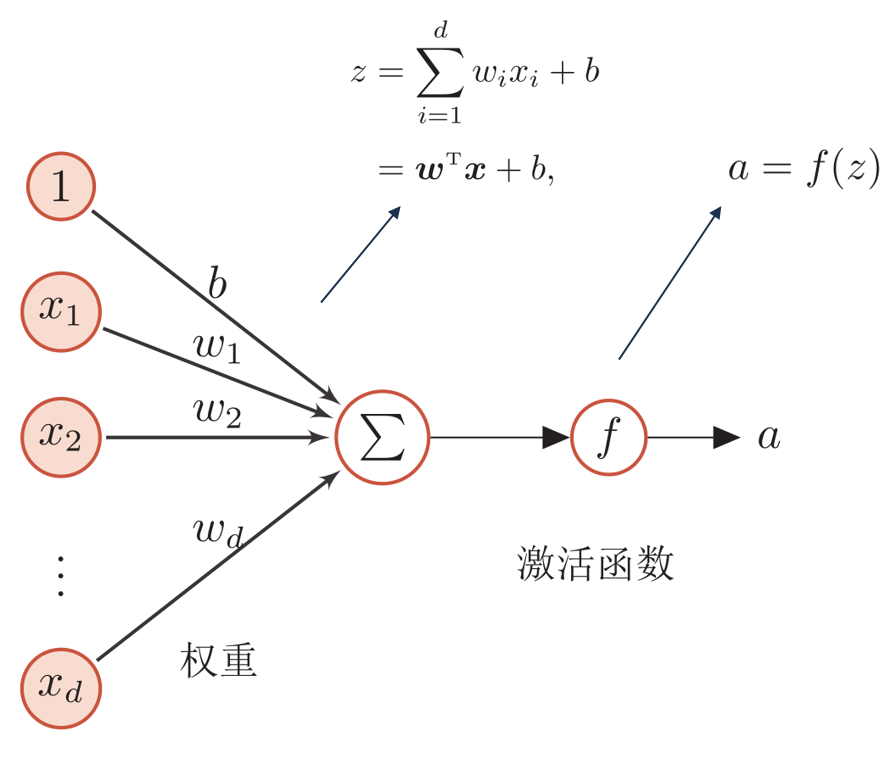
\includegraphics[width=0.6\linewidth]{人工神经元.png}
    \caption{人工神经元模型}
    \label{fig:神经元}
  \end{figure}

在图~\ref{fig:神经元}中,$\vec{x}$为输入向量,$w$和$b$分别是权重和偏移。

神经网络主要由以下几部分组成:
\begin{itemize}
    \item 输入节点(输入层)。在这一层中不进行任何计算,它们只是将信息传递给下一层(大部分时间是隐藏层)。
    \item 隐藏节点(隐藏层)。中间处理或计算在隐藏层中完成的,然后将输入层的权重(信号或信息)传递给下一层(另一个隐藏层或输出层)。一个神经网络也可以不包含隐藏层。
    \item 输出节点(输出层)。此层位于神经网络的最末层,负责接管来自前面隐藏层所输入的信息或信号。再通过激活函数,最终将得到合理范围内的理想数值,例如用于分类的softmax 函数。
    \item 连接和权重。神经元之间会有边进行连接,每条边会有一定的权重。即每个连接将神经元$i$的输出传递给神经元$j$的输入,每个连接被赋予一个权重$W_{ij}$。
    \item 激活函数。这个函数的作用在于将非线性特征引入到神经网络当中。同时它会将值的范围紧缩至更小,所以一个Sigmoid 激活函数的值区间为[0,1]。深度学习中有很多激活函数,如Sigmoid、Tanh、ReLU 、Softplus、Softmax 等。表\ref{table:激活函数}为常见的激活函数。
    \begin{table}[]
        \caption{激活函数}
        \label{table:激活函数}
        \centering
        \begin{tabular}{|l|l|l|}
        \hline
        名称&表达式&导数\\ \hline
        Sigmoid &  $f(x) = \frac{1}{1+e^{-x}}$ & $f'(x) = f(x)(1-f(x))$
        \\ \hline
        Tanh & $f(x) = \frac{2}{1+e^{-2x}} - 1$ & $f'(x) = 1 - f(x)^2$ \\ \hline
        ReLU & $f(x) = max(0, x)$ & $f'(x)=\begin{cases}
        0& \text{x<0}\\
        1& \text{x>=0}
        \end{cases}$ \\ \hline
        Softplus & $f(x) = log(1+e^x)$ & $f'(x) = \frac{e^x}{1+e^x}$ \\ \hline
        Softmax & $S_i = \frac{e_i}{\sum_j e_j}$ & \\ \hline
        \end{tabular}
        \end{table}
    \item 学习规则。利用学习规则修改神经网络中的权重和阈值。
\end{itemize}

\subsection{RNN}
% RNN是一种针对时序数据处理的神经网络模型。相较于普通的神经网络模型来说,更擅长处理序列数据,即该网络其具有短期记忆能力。在循环神经网络中,神经元不但可以接受其他神经元的信息,也可以接受自身的信息,形成具有环路的网络结构。

% 循环神经网络的通用近似定理[Haykin, 2009]: 如果一个完全
% 连接的循环神经网络有足够数量的sigmoid 型隐藏神经元,它可以以任意
% 的准确率去近似任何一个非线性动力系统

% 神经网络有很多类型,这里本文将神经网络划分为前馈神经网络和循环神经网络,其中前馈神经网络包含单层感知机、多层感知机(MLP)、卷积神经网络(CNN)等。
% 本文主要介绍循环神经网络, 循环神经网络(Recurrent Neural Network,RNN)是一类具有短期记忆能力的神经网络。.和前馈神经网络相比,循环神经网络更加符合生物神经网络的结构。
下图~\ref{fig:循环神经网络}是循环神经网络的示意图。
\begin{figure}
    \centering
    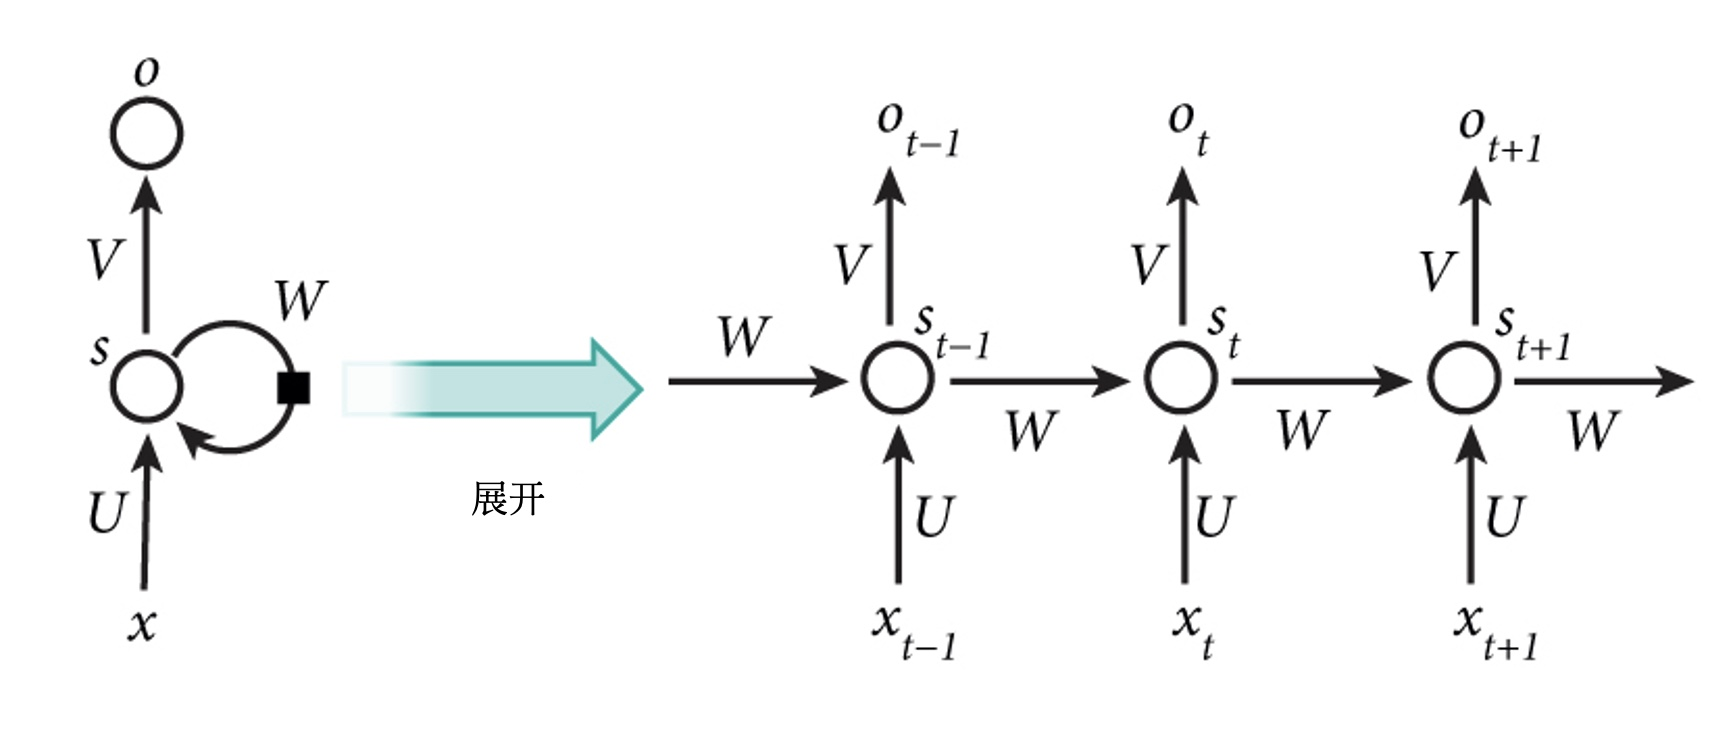
\includegraphics[width=0.6\linewidth]{循环神经网络.jpg}
    \caption{循环神经网络}
    \label{fig:循环神经网络}
  \end{figure}
该图显示了一个循环神经网络被展开成一个完整的神经网络。例如,如果输入序列是时间窗口为T的一组向量,那么网络会被展开成T层的神经网络。
  用公式表示如下:
  \begin{equation}
      \begin{aligned}
          O_t &= g(V\cdot S_t) \\
          S_t &= f(U\cdot X_t + W\cdot S_{t-1})
      \end{aligned}
  \end{equation}

  $x_t$表示第$t$步的输入,例如$x_1$表示时刻1的特征向量。$s_t$表示第t步隐藏层状态,也就是网络中的“记忆”。获得$s_t$的过程是计算位于之前的隐藏层状态及当前层的输入向量。函数$f(\cdot)$通常是一个非线性函数,如tanh或者ReLU。

RNN伪代码如算法\ref{RNN伪代码} 所示。
  \begin{algorithm}[!h]
    \caption{\emph{RNN伪代码}}
    \label{RNN伪代码}
    \begin{algorithmic}[1]
      \Require t时刻的特征向量
      \Ensure t+T时刻的特征向量
      \State 初始化t时刻单元状态
      \For{t $\leftarrow$ $1$ to $T$}
        \State $output_t = activation(input_t, state_t)$
        \State $state_t$ = $output_t$
      \EndFor
    \end{algorithmic}
  \end{algorithm}

\subsection{LSTM}
普通RNN有不能处理长依赖的问题,因此Hochreiter提出了一种长短期记忆网络-LSTM,LSTM是一种特殊的RNN,适用于学习长期依赖。现在LSTM已经被广泛应用于各个领域。LSTM和RNN类似,网络中都具有链式结构,但是LSTM中的循环单元与RNN中简单的$tanh$层不同,其构建了一些“门”(Gate)。利用构建出的“门”单元,能够将历史信息保留在当前节点状态,具体来说,是保留那些权重高的单元删除权重低的单元。
% 让神经网络记住很久之前的重要信息或者忘记最近的不重要信息。

% 所有RNN都具有链式形式。在普通的RNN中,这种循环是一种非常简单的结构,比如简单的tanh层。
\begin{figure}
    \centering
    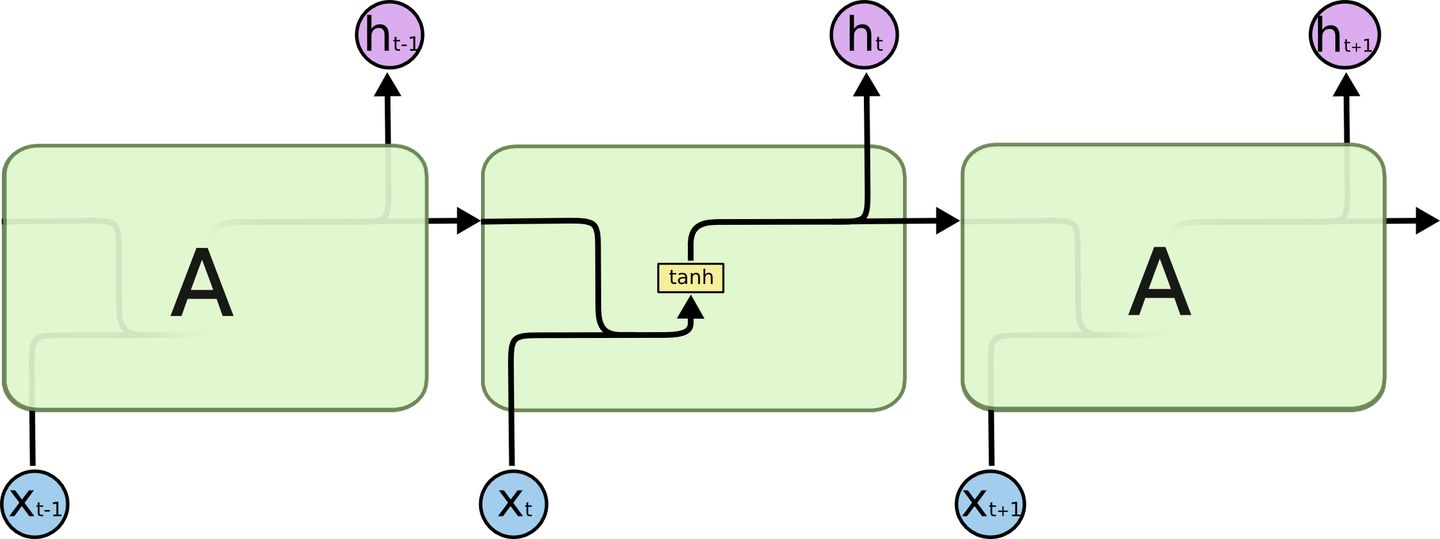
\includegraphics[width=0.6\linewidth]{普通RNN结构.jpg}
    \caption{普通RNN结构}
    \label{fig:普通RNN结构}
  \end{figure}

% LSTM也具有这种链式结构,但循环单元里面不再是只有单一的神经网络层,而是构建了一些“门”(Gate)。原来的 RNN,由于这种链式结构的限制,很长的时刻以前的输入对现在的网络影响非常小,后向传播时那些梯度也很难影响很早以前的输入,即会出现梯度消失的问题。而 LSTM 通过构建“门”,让网络能记住那些非常重要的信息,比如遗忘门,来选择性清空过去的记忆和更新较新的信息。
\begin{figure}
    \centering
    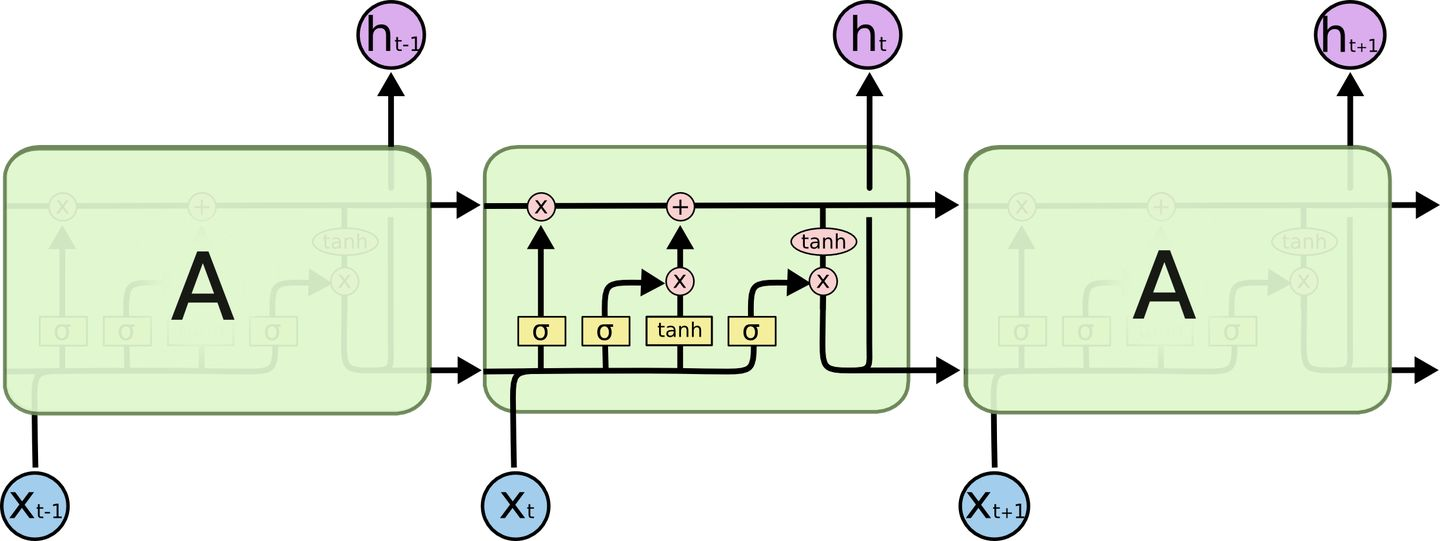
\includegraphics[width=0.6\linewidth]{LSTM结构.jpg}
    \caption{LSTM结构}
    \label{fig:LSTM结构}
  \end{figure}
  LSTM 首先通过$\sigma$层的“遗忘门”从单元状态中丢弃不重要的信息。遗忘门会读取上一时刻的输出$h_{t-1}$和当前时刻的输入$x_t$,计算出一个维度为n的向量$f_t$,该向量的值均在$[0, 1]$之间。1 表示“完全保留”上个神经元的状态信息,0 表示“完全舍弃”。

\begin{equation}
    \begin{aligned}
        f_t = \sigma(W_f\cdot x_t + U_f\cdot h_{t-1} + b_f)
    \end{aligned}
\end{equation}

下一步是确定该神经元的哪些新状态信息被存放在单元状态中。这里包含两个部分。第一,sigmoid 层,即 “输入门层” ,决定LSTM单元将更新哪些值。然后, tanh 层创建一个新的候选值$z_t$的向量,该向量可以加入到下一层单元状态中。

\begin{equation}
    \begin{aligned}
        i_t = \sigma(W_i\cdot[h_{t-1},x_t] + b_i)
    \end{aligned}
\end{equation}

\begin{equation}
    \begin{aligned}
        \widetilde {C_t} = tanh(W_C\cdot[h_{t-1},x_t]+b_C)
    \end{aligned}
\end{equation}
最后一步是将旧单元状态$c_{t-1}$更新为新状态$c_t$。把旧状态与遗忘门$f_t$相乘,丢弃掉之前无需保留的信息,接着与新状态进行相加,综合得出该神经元的输出的状态,也即更新单元的状态。
\begin{equation}
    \begin{aligned}
        C_t = f_t * C_{t-1} + i_t * \widetilde{C_t}
    \end{aligned}
\end{equation}


\begin{algorithm}[!h]
  \caption{\emph{LSTM伪代码}}
  \begin{algorithmic}[1]
      \Require 一组按时间排列的向量组
      \Ensure 按时间排列的向量组
      \State $\vec C_0 = \vec 0$
      \State $\vec h_0 = \vec 0$
      \For{$t$ \leftarrow $1$ to $T$}
      \State $output_t = activation(dot(W, input_t) + dot(U, state_t) + b)$
      \State $state_t = output_t$
      \State $i_t = activation(dot(state_t,))$
      % output_t = activation(dot(state_t, Uo) + dot(input_t, Wo) + dot(C_t, Vo) + bo)
      % #输入门
      % i_t = activation(dot(state_t, Ui) + dot(input_t, Wi) + bi)
      % 遗忘门
      % f_t = activation(dot(state_t, Uf) + dot(input_t, Wf) + bf)
      % #候选记忆单元
      % k_t = activation(dot(state_t, Uk) + dot(input_t, Wk) + bk)
      
      % c_t+1 = i_t * k_t + c_t * f_t

      \EndFor
  \end{algorithmic}
\end{algorithm}


\subsection{GRU}
门控循环单元(Gated Recurrent Unit,GRU)简化了LSTM模型,不仅合并了遗忘门和输入门,也合并了单元状态和隐藏层状态,在保证训练效果的同时大大减少了参数数量。
% 循环门单元(Gated Recurrent Unit,GRU),由 Cho, et al. (2014)提出。它组合了遗忘门和输入门到一个单独的“更新门”中。它也合并了cell state和hidden state,并且做了一些其他的改变。结果模型比标准LSTM模型更简单,
\begin{figure}
    \centering
    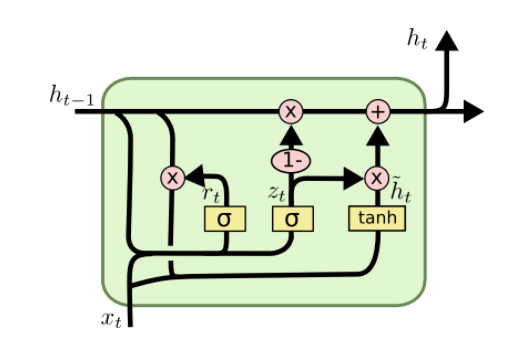
\includegraphics[width=0.6\linewidth]{GRU结构.png}
    \caption{GRU结构}
    \label{fig:GRU结构}
  \end{figure}

  \begin{equation}
    \begin{aligned}
        z_t = \sigma(W_z\cdot [h_{t-1},x_t])
    \end{aligned}
\end{equation}

\begin{equation}
    \begin{aligned}
        r_t = \sigma(W_r\cdot[h_{t-1},x_t])
    \end{aligned}
\end{equation}

\begin{equation}
    \begin{aligned}
        \widetilde {h_t} = tanh(W\cdot[r_t * h_{t-1}, x_t])
    \end{aligned}
\end{equation}

\begin{equation}
    \begin{aligned}
        h_t = (1- z_t) * h_{t-1} + z_t * \widetilde{h_t}
    \end{aligned}
\end{equation}
由图中结构可以看出,GRU是通过一个循环神经网络和“门”机制来不断更新内部参数。
% GRU算法的伪代码如下表所示。\ref{alg}

% \begin{algorithm}[!h]
%     \caption{\emph{GRU}}
%     \label{alg}
%     \begin{algorithmic}[1]
%       \Require
%         t

%       \Ensure
%         内部参数
%       \State 初始化t时刻单元状态
%       \For{t $\leftarrow$ $1$ to $T$}
%         \State $output_t$ = t
%         \State $state_t$ = $output_t$
%       \EndFor
%     % %   \While {$\mathcal{L}$没有收敛}
%     %       \State 利用公式 计算每一个节点$v$的$q_\phi(\bm{y}_v | \bm{A}, \bm{X}, Y_L)$以及$h_v^{K-1}$
%     %       \For{i $\leftarrow$ $1$ to $m$}
%     %       \State 从分布$q_\phi(Y_U | \bm{A}, \bm{X}, Y_L)$中采样$Y_U$
%     %       \State 在采样得到的$Y_U$基础上,利用公式计算$q_\phi(\bm{z}| \bm{A}, \bm{X}, Y)$ 
%     %        \For{j $\leftarrow$ $1$ to $n$}
%     %        \State 从分布$q_\phi(\bm{z}| \bm{A}, \bm{X}, Y)$ 中采样$\bm{z}$
%     %        \State 在采样得到的$\bm{z}$基础上用公式 计算$p_{\theta}(\bm{y}_v|\bm{A}, \bm{X}, \bm{z})$
%     %        \EndFor
%     %       \EndFor
%     %       \State 用公式计算目标函数$\mathcal{L}(\theta, \phi)$ 
%     %       \State 用梯度下降法更新$q_{net1}$,$q_{net2}$和$p_{net}$的所有参数
%     %   \EndWhile
%       %\State \Return $P_{net}$
%     \end{algorithmic}
%   \end{algorithm}


\section{基于关系图结构的RNN}
由前两节分析可知,LSTM和GRU作为两种循环神经网络,都可以很好地提取时序相关性。但是在复杂的清华大学校园网流量环境下,仍然有很多改进空间。根据第3章的实验结果,LSTM和GRU在CAMPUS数据集下准确率仅为65.4\%和67.8\%。经过特征分析,我们发现不同时刻下特征之间的相关性会发生变化。因此本文中我们利用循环神经网络(RNN)对时间依赖性进行建模的同时对特征关系也进行建模。值得指出的是,本文中使用的RNN子类是“门控循环单元”(GRU),相比于普通RNN,它可以很好地捕捉到时序数据中相隔较远的依赖关系。在GRU的矩阵乘法中,我们加入了前文提到的特征关系图(Feature Graph)。

定义无向权重图$G=(V,E,W)$,其中$V$表示特征节点的集合,$|V|=N$; $E$表示特征间的关联关系,即图中的边;$W \in R[N*N]$为特征节点的相似度的加权邻接矩阵,我们称$W$为特征关系矩阵。将时刻t观察到的流量特征向量表示为$X^t$。那么流量预测目的就是:给定$G$下,学得一个函数将$T$个历史图信号映射到未来$T$时刻的图信号:
\begin{equation}
    h[X^{t-T+1}, X^{t-T+2},...,X^{t}; G] \Rightarrow [X^{t+1}, X^{t+2}, ..., X^{t+T}]
\end{equation}

\begin{equation}
    r^{(t)} = \sigma(\Theta_r\star G[X^{(t)},H^{t-1}] + b_r)
\end{equation}

\begin{equation}
    u^{(t)} = \sigma(\Theta_u\star G[X^{(t)},H^{t-1}] + b_u)
\end{equation}

\begin{equation}
    C^{(t)} = tanh(\Theta_C\star_G[X^{(t)},(r^{(t)}\odot H^{(t-1)})] + b_c)
\end{equation}

\begin{equation}
    H^{(t)} = u^{(t)}\odot H^{(t-1)} + (1 - u^{(t)}) \odot C^{(t)}
\end{equation}

其中$X^{(t)}$, $H^{(t)}$表示在时间 $t$ 的输入和输出,$r^{(t)}$ $u^{(t)}$分别是在时间 $t$的复位门和更新门。$\star G$  表示扩散卷积,并且  是对应滤波器的参数。与GRU相似,该模型可用于构建递归神经网络层,并使用反向传播进行训练。
FG-RNN算法的原理如图\ref{fig:FG-RNN原理图}所示。
\begin{figure}[H]
  \centering
  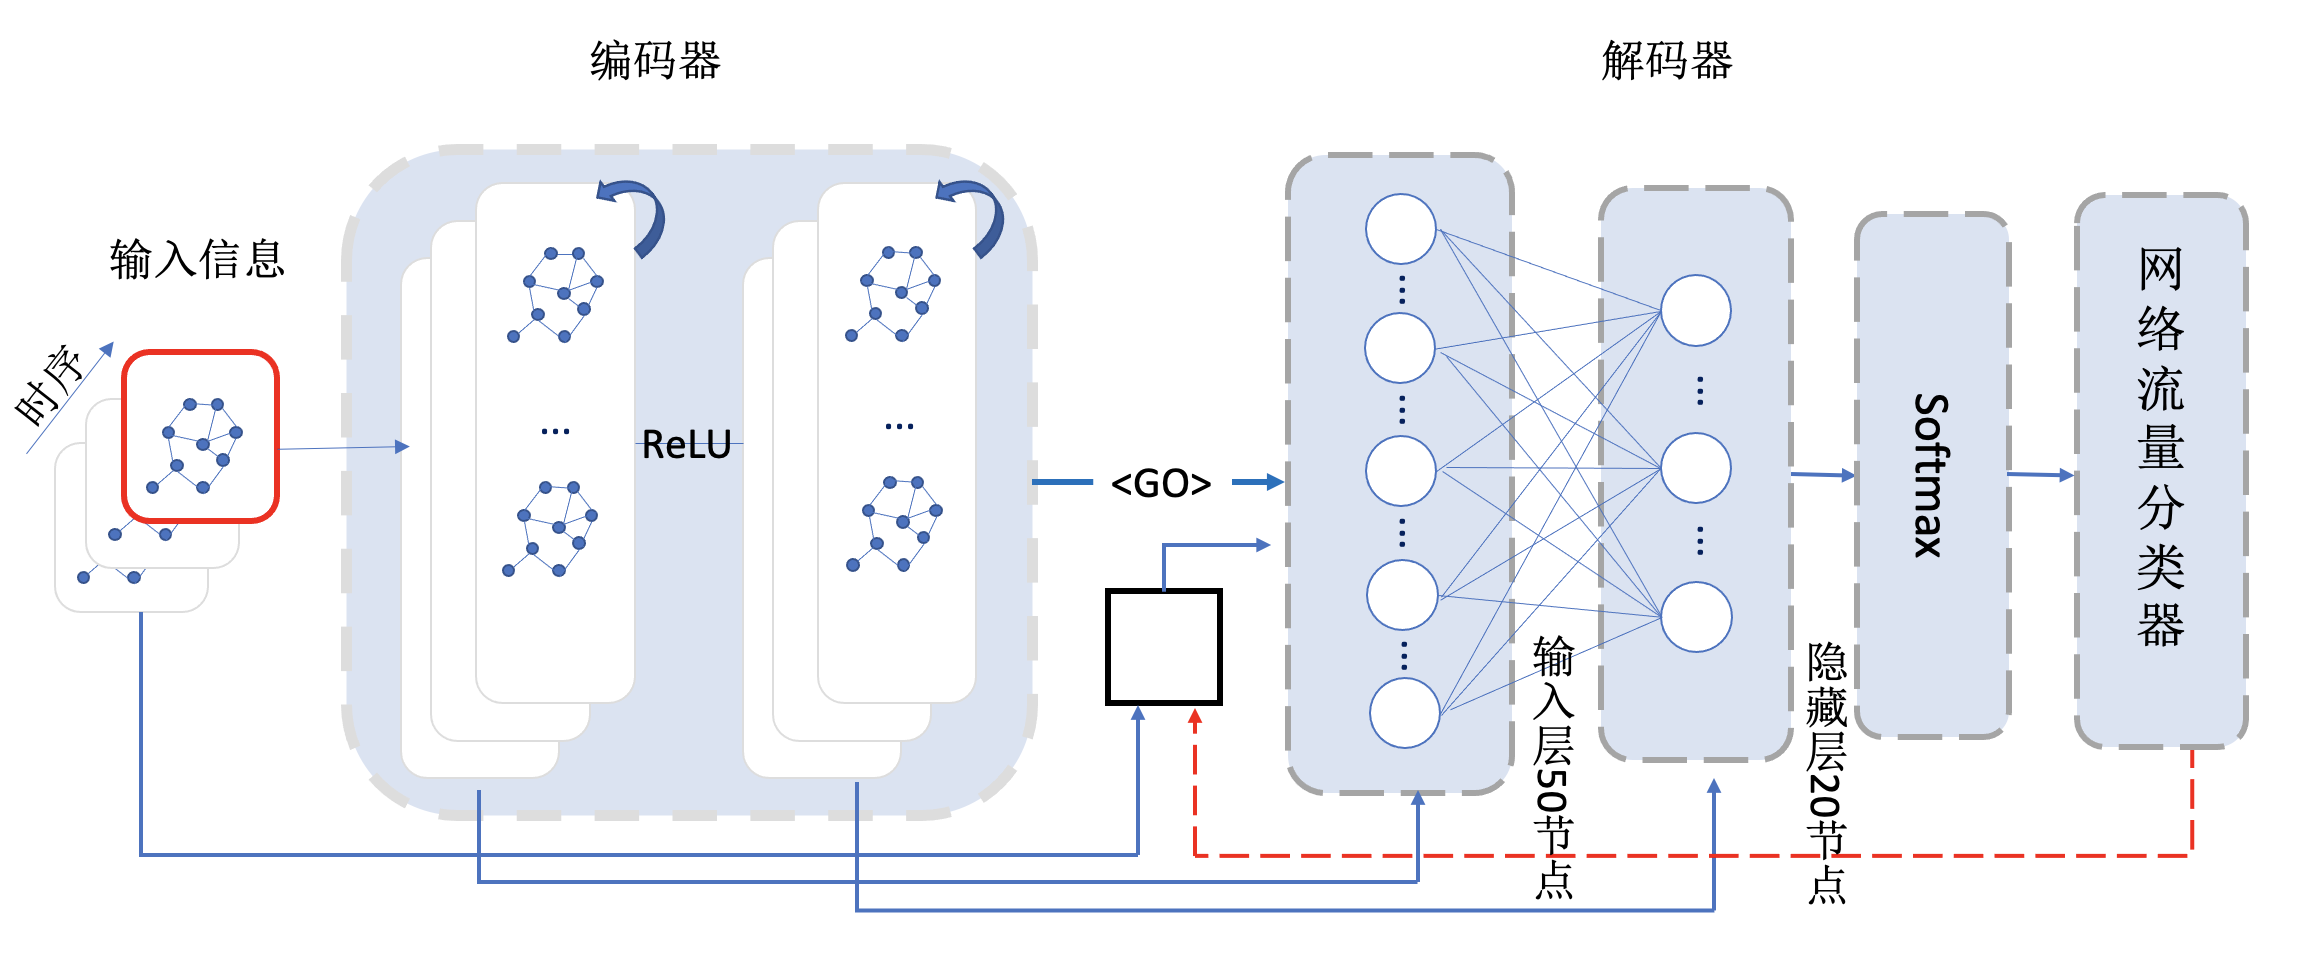
\includegraphics[width=1\linewidth]{FG-RNN原理图.png}
  \caption{FG-RNN原理图}
  \label{fig:FG-RNN原理图}
\end{figure}
FG-RNN算法的伪代码如算法\ref{FG-RNN伪代码}所示。
\begin{algorithm}[!h]
  \caption{\emph{FG-RNN伪代码}}
  \label{FG-RNN伪代码}
  \begin{algorithmic}[1]
    \Require
      一组按时间排序的向量组$\vec{x_1}$,$\vec{x_2}$,...,$\vec{x_T}$, 特征间关系图$G$以及它的邻接矩阵$W$

    \Ensure
      按时间排序的向量组$\vec{h_1}$,$\vec{h_2}$,...,$\vec{h_T}$
    \State 通过Xavier方法初始化$q_{net1}$, $q_{net2}$ and $p_{net}$的所有参数
    \While {$\mathcal{L}$没有收敛}
        \State 利用公式 计算每一个节点$v$的$q_{net1}$, $q_{net2}$ and $p_{net}$
        \For{i $\leftarrow$ $1$ to $T$}
        \State 更新特征关系矩阵$W(e)$的系数
        \State 更新GRU中的参数$W(X)$
        \State 计算$tanh(W(e) + W(X) + b)$        
        \EndFor
        \State 用公式计算目标函数$\mathcal{L}(\theta, \phi)$ 
        \State 用梯度下降法更新$q_{net1}$,$q_{net2}$和$p_{net}$的所有参数
    \EndWhile
    %\State \Return $P_{net}$
  \end{algorithmic}
\end{algorithm}

通常,计算卷积会很费时。 但是,如果$G$很稀疏,则可以使用总时间复杂度 $O(K \mid \varepsilon \mid) \ll O(N^ 2)$ 递归稀疏矩阵乘法来有效地进行计算,本文中计算特征关系图和GRU都可以使用该矩阵乘法。


% 循环神经网络解决了这个问题。它们是带有循环的网络,允许信息持续存在。循环神经网络可以被认为是同一个网络的多个副本,每个副本都会向后继者传递信息。
% \section{实验方案设计及实验流程}
% \begin{equation*} hl=[hl_{1},\ hl_{2},\ \ldots,\ hl_{n-f+1}] \tag{-} \end{equation*}

\section{在RNN中引入特征图信息}
在RNN的训练过程中,加入有效的额外辅助信息往往能够提升训练效果,例如在机器翻译领域,加入文章的关键词、摘要、作者信息等。通常加入信息的方式有以下几种。

\begin{enumerate}
  \item 直接将额外信息向量与当前特征向量叠加。原向量为$p=(p_1,p_2,...,p_n)$,额外信息向量为$e=(e_1,e_2,...,e_n)$,最终输入向量为$w=(p_1+e_1,p_2+e_2,...,p_n+e_n)$。这种方法需要保证额外信息向量与原向量维度相同。
  \item 将额外信息向量与当前特征向量拼接。原向量为$p=(p_1,p_2,...,p_n)$,额外信息向量为$e=(e_1,e_2,...,e_m)$,最终输入向量为$w=(p_1,p_2,...,p_n,e_1,e_2,...,e_m)$。也就是增加输入的维度,缺点是通常要求额外信息的特征与原特征类型保持一致,例如均为词向量。
  \item 增加一个额外的隐藏层,分别使用不同的矩阵进行变化,将结果用$tanh$函数映射到所需的维度。相当于增加一个普通循环神经网络模型和额外信息模型的感知器,然后加载到输出层上。即:
  \begin{equation}
    h'_t= tanh(W(p_t) + W(e) + b^{h'_t})
  \end{equation}
\end{enumerate}
因此,本文采用第三种方式将额外的特征关系图信息与原有特征结合起来。

\section{算法性能评估}
为了验证FG-RNN模型的有效性,本节首先在清华大学无线校园网真实场景下的数据集上开展有效性评估,随后在异常检测领域下的两个经典的公开数据集上进行实验,分别对比了FG-RNN和多个模型的评估效果,最后分析了模型参数的敏感性。


\subsection{训练过程对比}
图\ref{fig:随着训练轮次的增加准确率的变化}中横坐标为FG-RNN和LSTM两个算法随训练轮次的增加,准确率的变化,可以看出LSTM训练时间更短,大约25轮即可稳定,而FG-RNN需要训练50轮以上。

\begin{figure}[H]
    \centering
    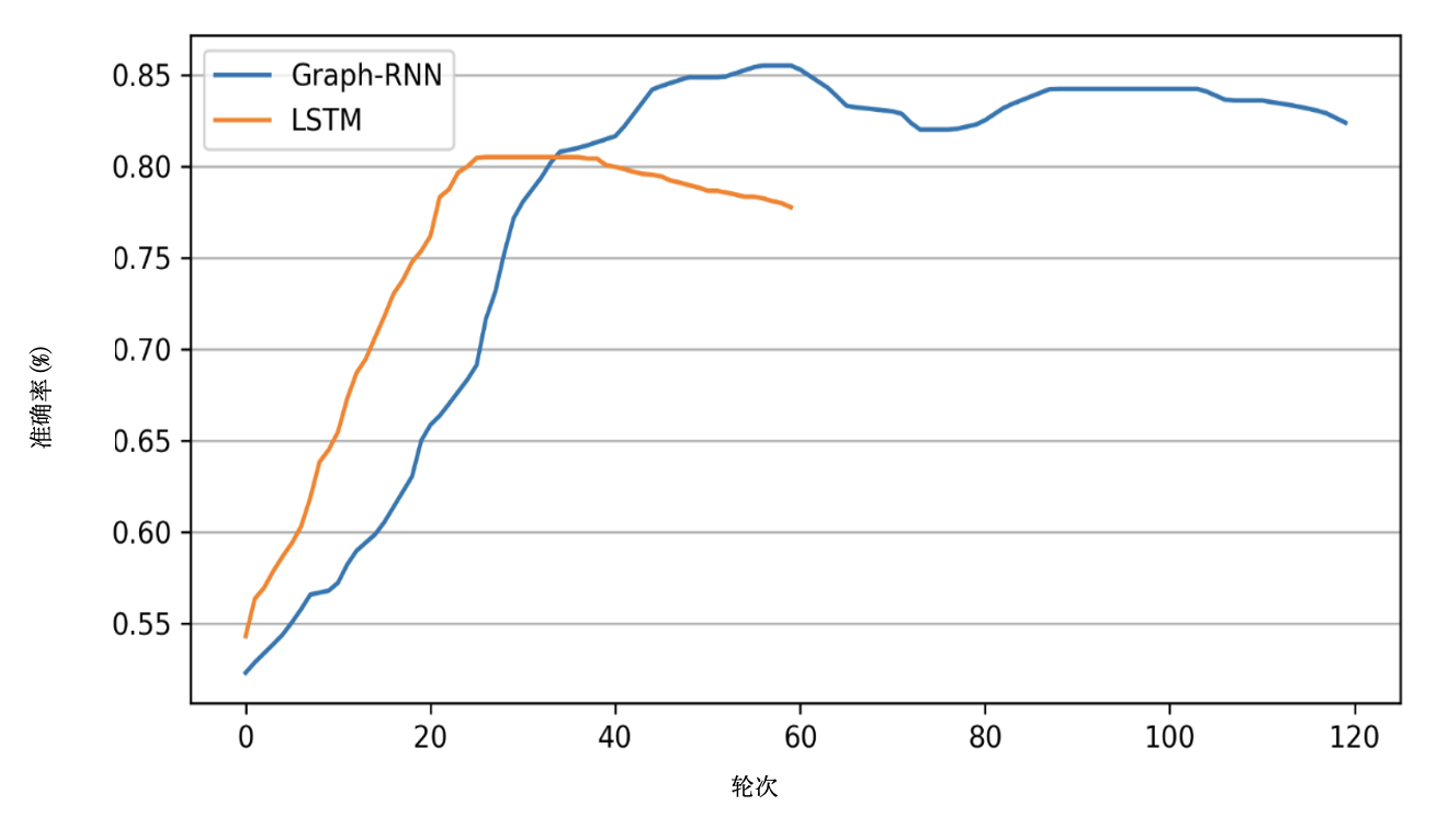
\includegraphics[width=1\linewidth]{accuracy_epoches.png}
    \caption{随着训练轮次的增加准确率的变化}
    \label{fig:随着训练轮次的增加准确率的变化}
  \end{figure}

图\ref{fig:loss收敛对比}表示FG-RNN和LSTM两个算法loss收敛的对比,在达到稳定的准确率后,loss也会维持一个相对稳定的水平。
  \begin{figure}[H]
    \centering
    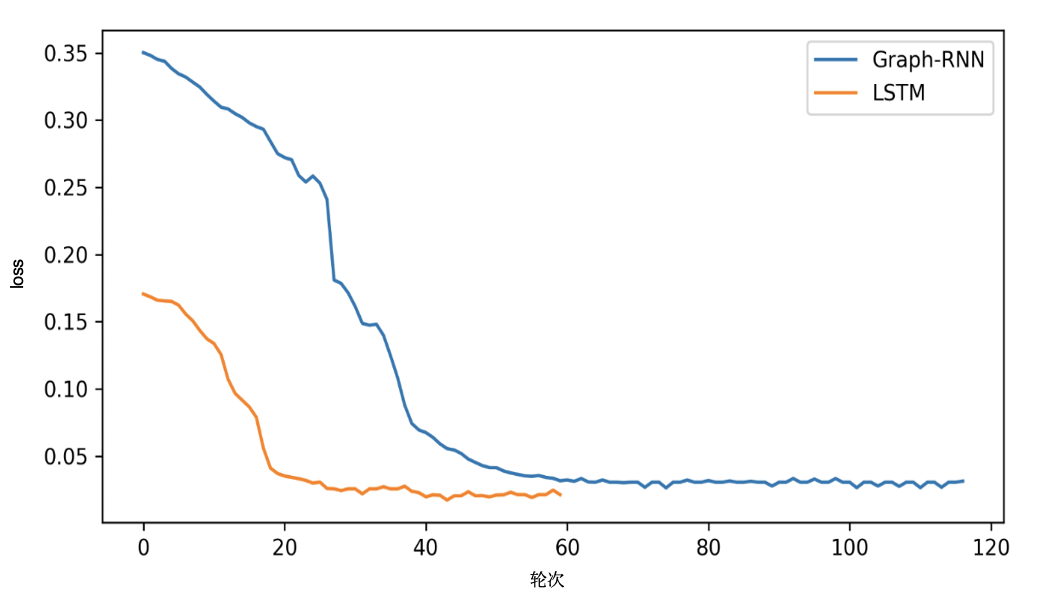
\includegraphics[width=1\linewidth]{loss_epoch.png}
    \caption{loss收敛对比}
    \label{fig:loss收敛对比}
  \end{figure}

\subsection{实验结果对比}

根据第3章的实验结果,LSTM和GRU在CAMPUS数据集下准确率仅为65.4\%和67.8\%,而加入固定的特征关系图后,LSTM准确率即可达到81.2\%,将特征关系图与RNN同时训练,动态更新特征关系矩阵的参数,则FG-RNN算法的准确率可达到85.3\%。

% \begin{algorithm}
%     \caption{A}
%     \label{alg:A}
%     % \begin{algorithmic}
%     \STATE {set $r(t)=x(t)$} 
%     \REPEAT 
%     \STATE set $h(t)=r(t)$ 
%     \REPEAT
%     \STATE set $h(t)=r(t)$ 
%     \UNTIL{B} 
%     \UNTIL{B}
%     % \end{algorithmic}
%     \end{algorithm}





%   \begin{algorithm}[!h]
%     \caption{\emph{GSNN}}
%     \label{alg}
%     \begin{algorithmic}[1]
%       \Require
%         图$G$以及它的邻接矩阵$A$,节点特征矩阵$X$以及已知节点的标签信息$T_L$,采样得到的$Y_U$和$\bm{z}$的数量:$m$和$n$

%       \Ensure
%         优化后的$q_{net1}$, $q_{net2}$和$p_{net}$所有参数
%       \State 通过Xavier方法\cite{glorot2010understanding}初始化$q_{net1}$, $q_{net2}$ and $p_{net}$的所有参数
%       \While {$\mathcal{L}$没有收敛}
%           \State 利用公式 \ref{seven} 计算每一个节点$v$的$q_\phi(\bm{y}_v | \bm{A}, \bm{X}, Y_L)$以及$h_v^{K-1}$
%           \For{i $\leftarrow$ $1$ to $m$}
%           \State 从分布$q_\phi(Y_U | \bm{A}, \bm{X}, Y_L)$中采样$Y_U$
%           \State 在采样得到的$Y_U$基础上,利用公式 \ref{eight}计算$q_\phi(\bm{z}| \bm{A}, \bm{X}, Y)$ 
%            \For{j $\leftarrow$ $1$ to $n$}
%            \State 从分布$q_\phi(\bm{z}| \bm{A}, \bm{X}, Y)$ 中采样$\bm{z}$
%            \State 在采样得到的$\bm{z}$基础上用公式\ref{nine} 计算$p_{\theta}(\bm{y}_v|\bm{A}, \bm{X}, \bm{z})$
%            \EndFor
%           \EndFor
%           \State 用公式\ref{ten}计算目标函数$\mathcal{L}(\theta, \phi)$ 
%           \State 用梯度下降法更新$q_{net1}$,$q_{net2}$和$p_{net}$的所有参数
%       \EndWhile
%       %\State \Return $P_{net}$
%     \end{algorithmic}
%   \end{algorithm}
% \subsection{基于开源数据集的检测结果}
% \begin{figure}
%   \centering
%   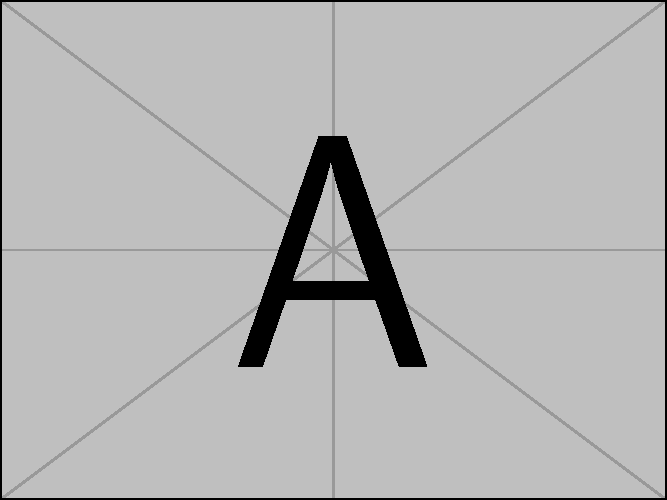
\includegraphics[width=0.6\linewidth]{example-image-a.pdf}
%   \caption{Example figure}
%   \label{fig:appendix-survey-figure}
% \end{figure}
% \begin{figure}
%   \centering
%   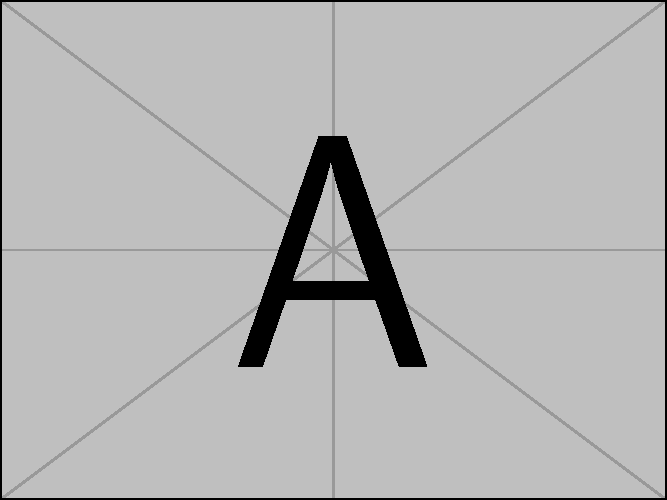
\includegraphics[width=0.6\linewidth]{example-image-a.pdf}
%   \caption{Example figure}
%   \label{fig:appendix-survey-figure}
% \end{figure}
% \subsection{基于真实数据的检测结果}
% 交叉熵损失函数经常用于分类问题中,特别是在神经网络做分类问题时,也经常使用交叉熵作为损失函数,此外,由于交叉熵涉及到计算每个类别的概率,所以交叉熵几乎每次都和sigmoid(或softmax)函数一起出现。

% 我们用神经网络最后一层输出的情况,来观察整个模型预测、获得损失和学习的流程:

% 神经网络最后一层得到每个类别的得分scores;
% 该得分经过sigmoid(或softmax)函数获得概率输出;
% 模型预测的类别概率输出与真实类别的one hot形式进行交叉熵损失函数的计算。
% \begin{figure}
%   \centering
%   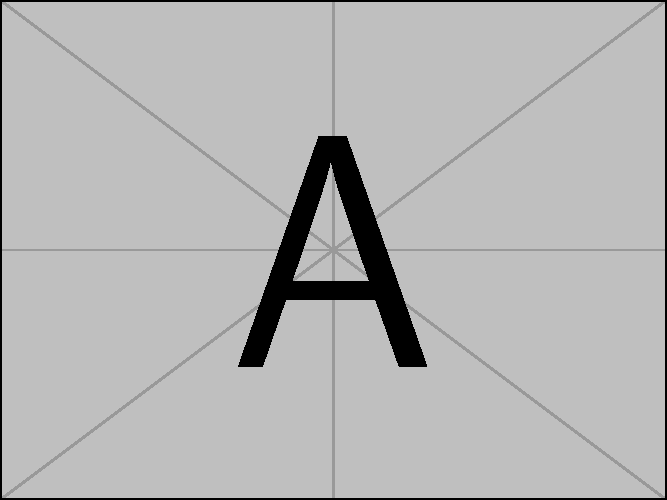
\includegraphics[width=0.6\linewidth]{example-image-a.pdf}
%   \caption{Example figure in appendix}
%   \label{fig:appendix-survey-figure}
% \end{figure}




